\documentclass[11pt,a4paper]{article}

% ==============================================================================
% Standard Packages (Overleaf & PDFLaTeX Compatible)
% ==============================================================================
\usepackage[utf8]{inputenc}
\usepackage[T1]{fontenc}
\usepackage[margin=1in]{geometry}
\usepackage{amsmath,amssymb,amsfonts}
\usepackage{graphicx}
\usepackage{booktabs}
\usepackage{caption}
\usepackage{microtype}
\usepackage{cite}
\usepackage{url}
\usepackage{xcolor}
\usepackage{tabularx}
\usepackage{array}
\usepackage{titlesec}
\usepackage[hidelinks,colorlinks=true,linkcolor=blue!75!black,citecolor=blue!75!black,urlcolor=blue!75!black]{hyperref}

% Section Heading Formatting
\titleformat{\section}{\large\bfseries}{\thesection.}{0.5em}{}
\titleformat{\subsection}{\normalsize\bfseries}{\thesubsection.}{0.5em}{}
\titleformat{\subsubsection}{\normalsize\itshape}{\thesubsubsection.}{0.5em}{}

% Clean Page Setup
\pagestyle{plain}

% ==============================================================================
% Document Title and Author Block
% ==============================================================================
\title{\Large\textbf{Comparative Evaluation of Large Language Models for Scientific Highlight Generation: Reference Quality, Source Grounding, and Runtime Efficiency}}

\author{%
  \textbf{Debarghya Bhowmick}$^{1,*}$, \textbf{Tohida Rehman}$^{2}$\\[0.8em]
  \small $^{1}$Department of Computer Science \& Engineering, I. K. Gujral Punjab Technical University, Kapurthala, Punjab, India\\
  \small Email: \texttt{debarghya.bhowmick@yahoo.com} \quad ORCID: \href{https://orcid.org/0009-0003-0468-8981}{0009-0003-0468-8981}\\[0.4em]
  \small $^{2}$Department of Information Technology, Jadavpur University, Kolkata, West Bengal, India\\
  \small Email: \texttt{tohidarehman.it@jadavpuruniversity.in} \quad ORCID: \href{https://orcid.org/0000-0002-3578-1316}{0000-0002-3578-1316}\\[0.6em]
  \small $^{*}$Corresponding author: \texttt{debarghya.bhowmick@yahoo.com}
}
\date{}

% ==============================================================================
% Main Document
% ==============================================================================
\begin{document}

\maketitle

\begin{abstract}
Reading and understanding new scientific discoveries has become increasingly difficult because thousands of research papers are published every single day. Most academic journals now require authors to write research highlights, which are short summary statements that explain the main findings of a paper in simple terms. In this research project, conducted as part of a research internship under the supervision of Dr. Tohida Rehman at Jadavpur University, we investigate how modern artificial intelligence models can automatically read a scientific abstract and generate accurate highlights. To test this, we used a large public collection of 13,825 academic papers from the FIRE MixSub-SciHigh dataset across medical, biological, and engineering fields. We evaluated four different types of language models: Google Pegasus-PubMed, BioMistral-7B, Qwen-2.5-Instruct, and Meta Llama-3.1-8B-Instruct. We evaluated these models across three key dimensions: how well they match human-written highlights, how strictly they stick to the facts without inventing false information, and how fast they run on standard computer hardware. Our experiments show that BioMistral-7B is the safest model for medical content because 84.44\% of its words come directly from the source text, keeping the risk of inventing unverified claims down to only 15.56\%. On the other hand, Qwen-2.5-Instruct achieved the highest similarity to human highlights and proved to be the fastest model, taking only 3.31 seconds per paper, which is more than twice as fast as the other systems. We also built an interactive web dashboard that allows users to test any paper and visually check which words are grounded in the source text.
\end{abstract}

\vspace{0.5em}
\noindent\textbf{Keywords:} Scientific highlight generation, Natural language processing, Large language models, Factuality, BioMistral, Qwen-2.5, Summarization.

\vspace{1em}

% ------------------------------------------------------------------------------
\section{Introduction}
\label{sec:intro}
% ------------------------------------------------------------------------------
Scientific research moves at an extraordinary pace. Every year, researchers publish hundreds of thousands of papers in computer science, medicine, physics, and biology \cite{fire2026mixsub}. For busy doctors, engineers, and students, reading complete papers or even full abstracts takes too much time. An abstract is often dense and contains background explanations, literature citations, and complex descriptions of experiments. Because of this, major academic publishers such as Elsevier and Springer Nature ask authors to write three to five short bullet points called research highlights. These highlights allow a reader to understand the novel findings of a study in less than thirty seconds.

Writing these highlights by hand requires careful effort from scientists. If artificial intelligence can read a scientific paper and create reliable highlights automatically, it could save countless hours of work and help search engines summarize papers for readers. However, summarizing a scientific paper is much harder than summarizing a newspaper article or a story \cite{maynez2020faithfulness}. Scientific papers contain specialized medical words, chemical names, and mathematical outcomes. If an artificial intelligence model makes a mistake or invents a fact that was not in the original paper, it can lead to dangerous misunderstandings.

In this work, which was carried out during a research internship under the mentorship of Dr. Tohida Rehman in the Department of Information Technology at Jadavpur University, we set out to study and compare different artificial intelligence models for this task. We selected the publicly accessible FIRE MixSub-SciHigh dataset \cite{fire2026mixsub}, which pairs scientific abstracts with real author-written highlights. We evaluated four models that represent different design approaches in modern natural language processing:
\begin{enumerate}
    \item Google Pegasus-PubMed, a classic sequence-to-sequence model designed specifically for medical text \cite{zhang2020pegasus}.
    \item BioMistral-7B, a large language model trained further on medical literature from PubMed Central \cite{labrak2024biomistral}.
    \item Qwen-2.5-Instruct, a modern, highly efficient instruction-following model \cite{yang2024qwen25}.
    \item Meta Llama-3.1-8B-Instruct, a widely used general-purpose open foundation model \cite{dubey2024llama3}.
\end{enumerate}

Rather than looking only at standard word-matching scores, we created a three-pillar evaluation system. First, we measured quality by checking how closely the model matches the human author's text. Second, we measured grounding by calculating whether the model sticks to the facts in the abstract or invents new words. Third, we measured speed by timing how long each model takes to generate highlights on a standard graphics processing unit. Finally, we turned our findings into an easy-to-use web application so that students, teachers, and researchers can test abstracts and examine the results in real time.

% ------------------------------------------------------------------------------
\section{Related Work}
\label{sec:related}
% ------------------------------------------------------------------------------
Automatic text summarization has been studied for decades in computer science. Early systems used extractive methods, which simply copy the most important sentences from the input text using statistical word counts or graph algorithms. While extractive summaries are safe from inventing false facts, they often sound disjointed and fail to synthesize multiple findings into clean, concise statements.

The field changed dramatically with the introduction of the Transformer architecture by Vaswani and colleagues \cite{vaswani2017attention}. This allowed models to read and generate text with much greater contextual awareness. Researchers developed sequence-to-sequence models like BART \cite{lewis2020bart}, T5 \cite{raffel2020t5}, and PEGASUS \cite{zhang2020pegasus}. PEGASUS introduced a pre-training technique called gap-sentence generation, where important sentences were removed from scientific papers and the model learned to fill them back in. When trained on PubMed articles, PEGASUS became a strong baseline for biomedical text summarization.

In recent years, the community has shifted toward decoder-only autoregressive language models containing billions of parameters \cite{yang2024qwen25, dubey2024llama3}. These models are trained on massive text collections and fine-tuned to follow user instructions. Because training huge models from scratch is expensive, researchers frequently adapt existing models to specific domains. For example, BioMistral \cite{labrak2024biomistral} was created by taking Mistral-7B and continuing its training on open-access papers from PubMed Central. Techniques like LoRA \cite{hu2022lora} and QLoRA \cite{dettmers2023qlora} further made it possible to run and adapt these models using 4-bit quantization on affordable hardware.

Despite these advancements, language models still suffer from hallucinations, which means generating text that sounds convincing but is factually unsupported \cite{maynez2020faithfulness}. In scientific fields, measuring hallucination is critical. In our internship research, we build upon these foundations by comparing domain-specific, general-purpose, and lightweight instruction models under strictly identical constraints.

% ------------------------------------------------------------------------------
\section{The Dataset}
\label{sec:dataset}
% ------------------------------------------------------------------------------
To carry out our experiments, we utilized the openly available scientific dataset from the FIRE MixSub-SciHigh shared task \cite{fire2026mixsub}. We used this dataset purely as a research benchmark for our internship project at Jadavpur University to test how well different language models perform on real scientific papers. The corpus contains a total of 13,825 academic publications from fields such as child psychology, oncology, dental materials, and computer science.

\begin{table}[htbp]
    \centering
    \caption{Dataset partitions and document statistics used in our benchmark.}
    \label{tab:dataset}
    \small
    \begin{tabular*}{\textwidth}{@{\extracolsep{\fill}}llcl@{}}
        \toprule
        \textbf{Split Name} & \textbf{Filename} & \textbf{Total Papers} & \textbf{Description} \\
        \midrule
        Training Set & \texttt{MixSub-SciHigh\_train\_FIRE.csv} & 10,000 & Papers with abstracts and gold author highlights \\
        Validation Set & \texttt{MixSub-SciHigh\_val\_FIRE.csv} & 1,985 & Held-out papers used for our three-pillar evaluation \\
        Masked Test Set & \texttt{MixSub-SciHigh\_test\_FIRE(Masked).csv} & 1,840 & Test papers with abstracts only for blind evaluation \\
        \bottomrule
    \end{tabular*}
\end{table}

Table~\ref{tab:dataset} summarizes the three parts of the dataset. The training split contains 10,000 papers. The validation split contains 1,985 papers, each containing the original paper abstract written by the authors and the human-written highlights. The masked test split contains 1,840 papers where only the abstract is provided.

In this dataset, each abstract typically contains between 200 and 350 words, describing the background of the study, what experiment was conducted, and what the scientists found. The corresponding highlights contain three to five short sentences, averaging 40 to 80 words in total. An example from the validation set shows what the input and output look like:
\begin{quote}
    \small
    \textbf{Sample Abstract:} \textit{``Standardized developmentally based assessment systems have transformed the capacity to identify transdiagnostic behavioral markers of mental disorder risk in early childhood notably clinically significant irritability... We measured children's facial muscular movement during a mildly frustrating task using automated Facial Action Coding...''}\\
    \textbf{Author Highlights:} \textit{``There is a need for tools that assess child irritability and externalizing behaviors. We measured childrens facial muscular movement during a mildly frustrating task. Negative expressions with eye contact differentiated children with clinical problems.''}
\end{quote}

% ------------------------------------------------------------------------------
\section{The Three-Pillar Evaluation Framework}
\label{sec:framework}
% ------------------------------------------------------------------------------
When evaluating computer-generated summaries, most past papers only reported word overlap scores like ROUGE \cite{lin2004rouge}. However, in real life, a model that gets a good word score might invent dangerous medical claims, or it might be so slow that nobody can afford to run it. To give a complete picture, we organized our evaluation into three simple pillars: quality, factual grounding, and speed.

\subsection{Pillar 1: Quality and Similarity to Human Highlights}
The first pillar asks whether the generated highlight matches what the human author wrote. We measure this in two ways:
\begin{enumerate}
    \item \textbf{ROUGE-L Score:} ROUGE-L looks for the longest common subsequence of words between the generated text and the human reference text \cite{lin2004rouge}. It checks how many words appear in the exact same relative order, even if there are other words in between:
    \begin{equation}
        P_{LCS} = \frac{LCS(\text{Generated}, \text{Reference})}{|\text{Generated}|}, \qquad R_{LCS} = \frac{LCS(\text{Generated}, \text{Reference})}{|\text{Reference}|}
    \end{equation}
    \begin{equation}
        ROUGE\text{-}L_{F1} = \frac{2 \times P_{LCS} \times R_{LCS}}{P_{LCS} + R_{LCS}}
    \end{equation}
    Here, a higher F1 score means the model captured both the important words and the overall structure of the human highlight.
    \item \textbf{Target Lexical F1:} This measures the basic word overlap between the unique words in the generated highlight and the unique words in the human reference:
    \begin{equation}
        P_{\text{target}} = \frac{|\text{Generated Words} \cap \text{Reference Words}|}{|\text{Generated Words}|}
    \end{equation}
    \begin{equation}
        F1_{\text{target}} = \frac{2 \times P_{\text{target}} \times R_{\text{target}}}{P_{\text{target}} + R_{\text{target}}}
    \end{equation}
\end{enumerate}

\subsection{Pillar 2: Factual Grounding and Hallucination Risk Proxy}
The second pillar checks whether the model stays faithful to the abstract or makes things up. If an artificial intelligence model generates words that were never in the source abstract, there is a risk that it is inventing information.
\begin{enumerate}
    \item \textbf{Source Lexical Precision ($P_{\text{source}}$):} This is the percentage of generated words that actually appeared in the source abstract:
    \begin{equation}
        P_{\text{source}} = \frac{|\text{Generated Words} \cap \text{Abstract Words}|}{|\text{Generated Words}|}
    \end{equation}
    For instance, if a model writes 100 words and 85 of those words were already in the abstract, the source precision is 85\%.
    \item \textbf{Ungrounded-Token Risk Proxy (\%):} This is simply the opposite of source precision:
    \begin{equation}
        \text{Risk Proxy (\%)} = (1.0 - P_{\text{source}}) \times 100
    \end{equation}
    A lower risk proxy is much better because it shows that the model is sticking closely to the provided text instead of bringing in outside vocabulary.
\end{enumerate}

\subsection{Pillar 3: Inference Speed and Efficiency}
The third pillar measures how fast the model runs. We recorded the actual clock time in seconds that each model took to read an abstract and generate its highlights:
\begin{equation}
    \text{Mean Latency} = \frac{1}{N} \sum_{i=1}^{N} T_i \quad (\text{seconds per paper})
\end{equation}
We also calculated how many papers the model can process per second (sample throughput) and how many words or tokens it creates per second (token speed). A model that produces high quality in three seconds is much more practical than a model that produces slightly higher quality but takes fifteen seconds.

% ------------------------------------------------------------------------------
\section{Experimental Setup}
\label{sec:setup}
% ------------------------------------------------------------------------------
To make sure our comparison was completely fair, we set identical rules for all models. We limited the input abstract length to 512 tokens so that every model had the same input window. We limited the output length to 128 tokens so that every model had to produce a short highlight rather than a long essay.

All experiments were conducted on a single computer equipped with an NVIDIA Tesla T4 graphics card with approximately 16 gigabytes of video memory. Large language models with seven or eight billion parameters are usually too large to fit into this amount of memory using standard precision. To solve this engineering challenge, we applied 4-bit NormalFloat4 (NF4) quantization using the \texttt{bitsandbytes} library \cite{dettmers2023qlora}. This compressed the memory footprint of the models down to roughly five gigabytes, allowing them to run smoothly without running out of memory.

For the three autoregressive models, we used a clear, standardized prompt asking the model to act as a scientific editor and generate concise highlights. For Pegasus-PubMed, we used its standard sequence-to-sequence generation pipeline. All evaluation scripts were written in Python using Hugging Face Transformers and the official ROUGE library.

% ------------------------------------------------------------------------------
\section{Results and Discussion}
\label{sec:results}
% ------------------------------------------------------------------------------
Table~\ref{tab:results} presents the complete results of our benchmark across all four models. These numbers come directly from our recorded evaluation files and reveal clear trade-offs between the different architectures.

\begin{table*}[t]
    \centering
    \caption{Complete Three-Pillar Benchmark Performance on the FIRE MixSub-SciHigh Validation Dataset.}
    \label{tab:results}
    \small
    \resizebox{\textwidth}{!}{%
    \begin{tabular}{@{}llccccccc@{}}
        \toprule
        \textbf{Model Architecture} & \textbf{Evaluation Mode} & \textbf{ROUGE-L} & \textbf{Target F1} & \textbf{Grounding} & \textbf{Risk Proxy} & \textbf{Mean Latency} & \textbf{Throughput} & \textbf{Token Speed} \\
        & & \textbf{F1 (\%)} & \textbf{(\%)} & \textbf{(\%)} & \textbf{(\% $\downarrow$)} & \textbf{(s/sample $\downarrow$)} & \textbf{(samp/s $\uparrow$)} & \textbf{(tok/s $\uparrow$)} \\
        \midrule
        \textbf{Qwen-2.5-Instruct} & Zero-shot (4-bit) & \textbf{19.87\%} & \textbf{28.27\%} & 59.49\% & 40.51\% & \textbf{3.31 s} & \textbf{0.302} & \textbf{28.19} \\
        \textbf{BioMistral-7B} & Zero-shot (4-bit) & 19.80\% & 27.37\% & \textbf{84.44\%} & \textbf{15.56\%} & 8.04 s & 0.124 & 12.69 \\
        \textbf{Llama-3.1-8B-Instruct} & Zero-shot (4-bit) & 19.04\% & 25.07\% & 53.40\% & 46.60\% & 7.90 s & 0.127 & --- \\
        \textbf{Pegasus-PubMed} & Seq2Seq Baseline & 16.90\% & 22.32\% & 57.40\% & 42.60\% & 10.56 s & 0.095 & 9.18 \\
        \bottomrule
    \end{tabular}}
\end{table*}

\subsection{Comparing Quality Across Models}
Looking at Pillar 1, the newer decoder-only language models clearly outperformed the older sequence-to-sequence model. Pegasus-PubMed scored 16.90\% on ROUGE-L F1, whereas Qwen-2.5-Instruct scored 19.87\% and BioMistral-7B scored 19.80\%. The difference between Qwen and BioMistral is only 0.07\%, which means both models were equally good at capturing the main ideas that human authors included in their highlights. Llama-3.1-8B was slightly behind at 19.04\%.

\subsection{Comparing Factual Safety and Grounding}
The results for Pillar 2 show a dramatic difference between general models and domain-trained models. BioMistral-7B was the clear winner in factual safety. A remarkable 84.44\% of the words it generated came directly from the provided abstract. This means its ungrounded risk proxy was only 15.56\%.

By contrast, Llama-3.1 had a risk proxy of 46.60\%, and Qwen-2.5 had a risk proxy of 40.51\%. Because Llama and Qwen are general-purpose models, they often rephrased findings using creative synonyms and editorial framing words that were not in the abstract. In clinical and medical research, using words that were never in the study can be risky. BioMistral stayed strictly grounded in the medical vocabulary of the abstract because it had been trained specifically on medical papers from PubMed Central.

\subsection{Comparing Speed and Processing Efficiency}
In Pillar 3, Qwen-2.5-Instruct proved to be significantly faster than all other systems. It generated highlights in just 3.31 seconds per paper, creating 28.19 tokens every second. In comparison, BioMistral took 8.04 seconds per paper, Llama-3.1 took 7.90 seconds, and Pegasus took 10.56 seconds. Qwen was roughly 2.4 times faster than BioMistral and Llama, and more than 3 times faster than Pegasus. In a production system where a digital library needs to summarize thousands of new papers every evening, Qwen would finish the job in less than half the time required by the other models.

% ------------------------------------------------------------------------------
\section{Visual Analysis of Results}
\label{sec:visuals}
% ------------------------------------------------------------------------------
To make these numerical comparisons easy to understand visually, we created four charts that illustrate the trade-offs between the pillars.

\begin{figure}[htbp]
    \centering
    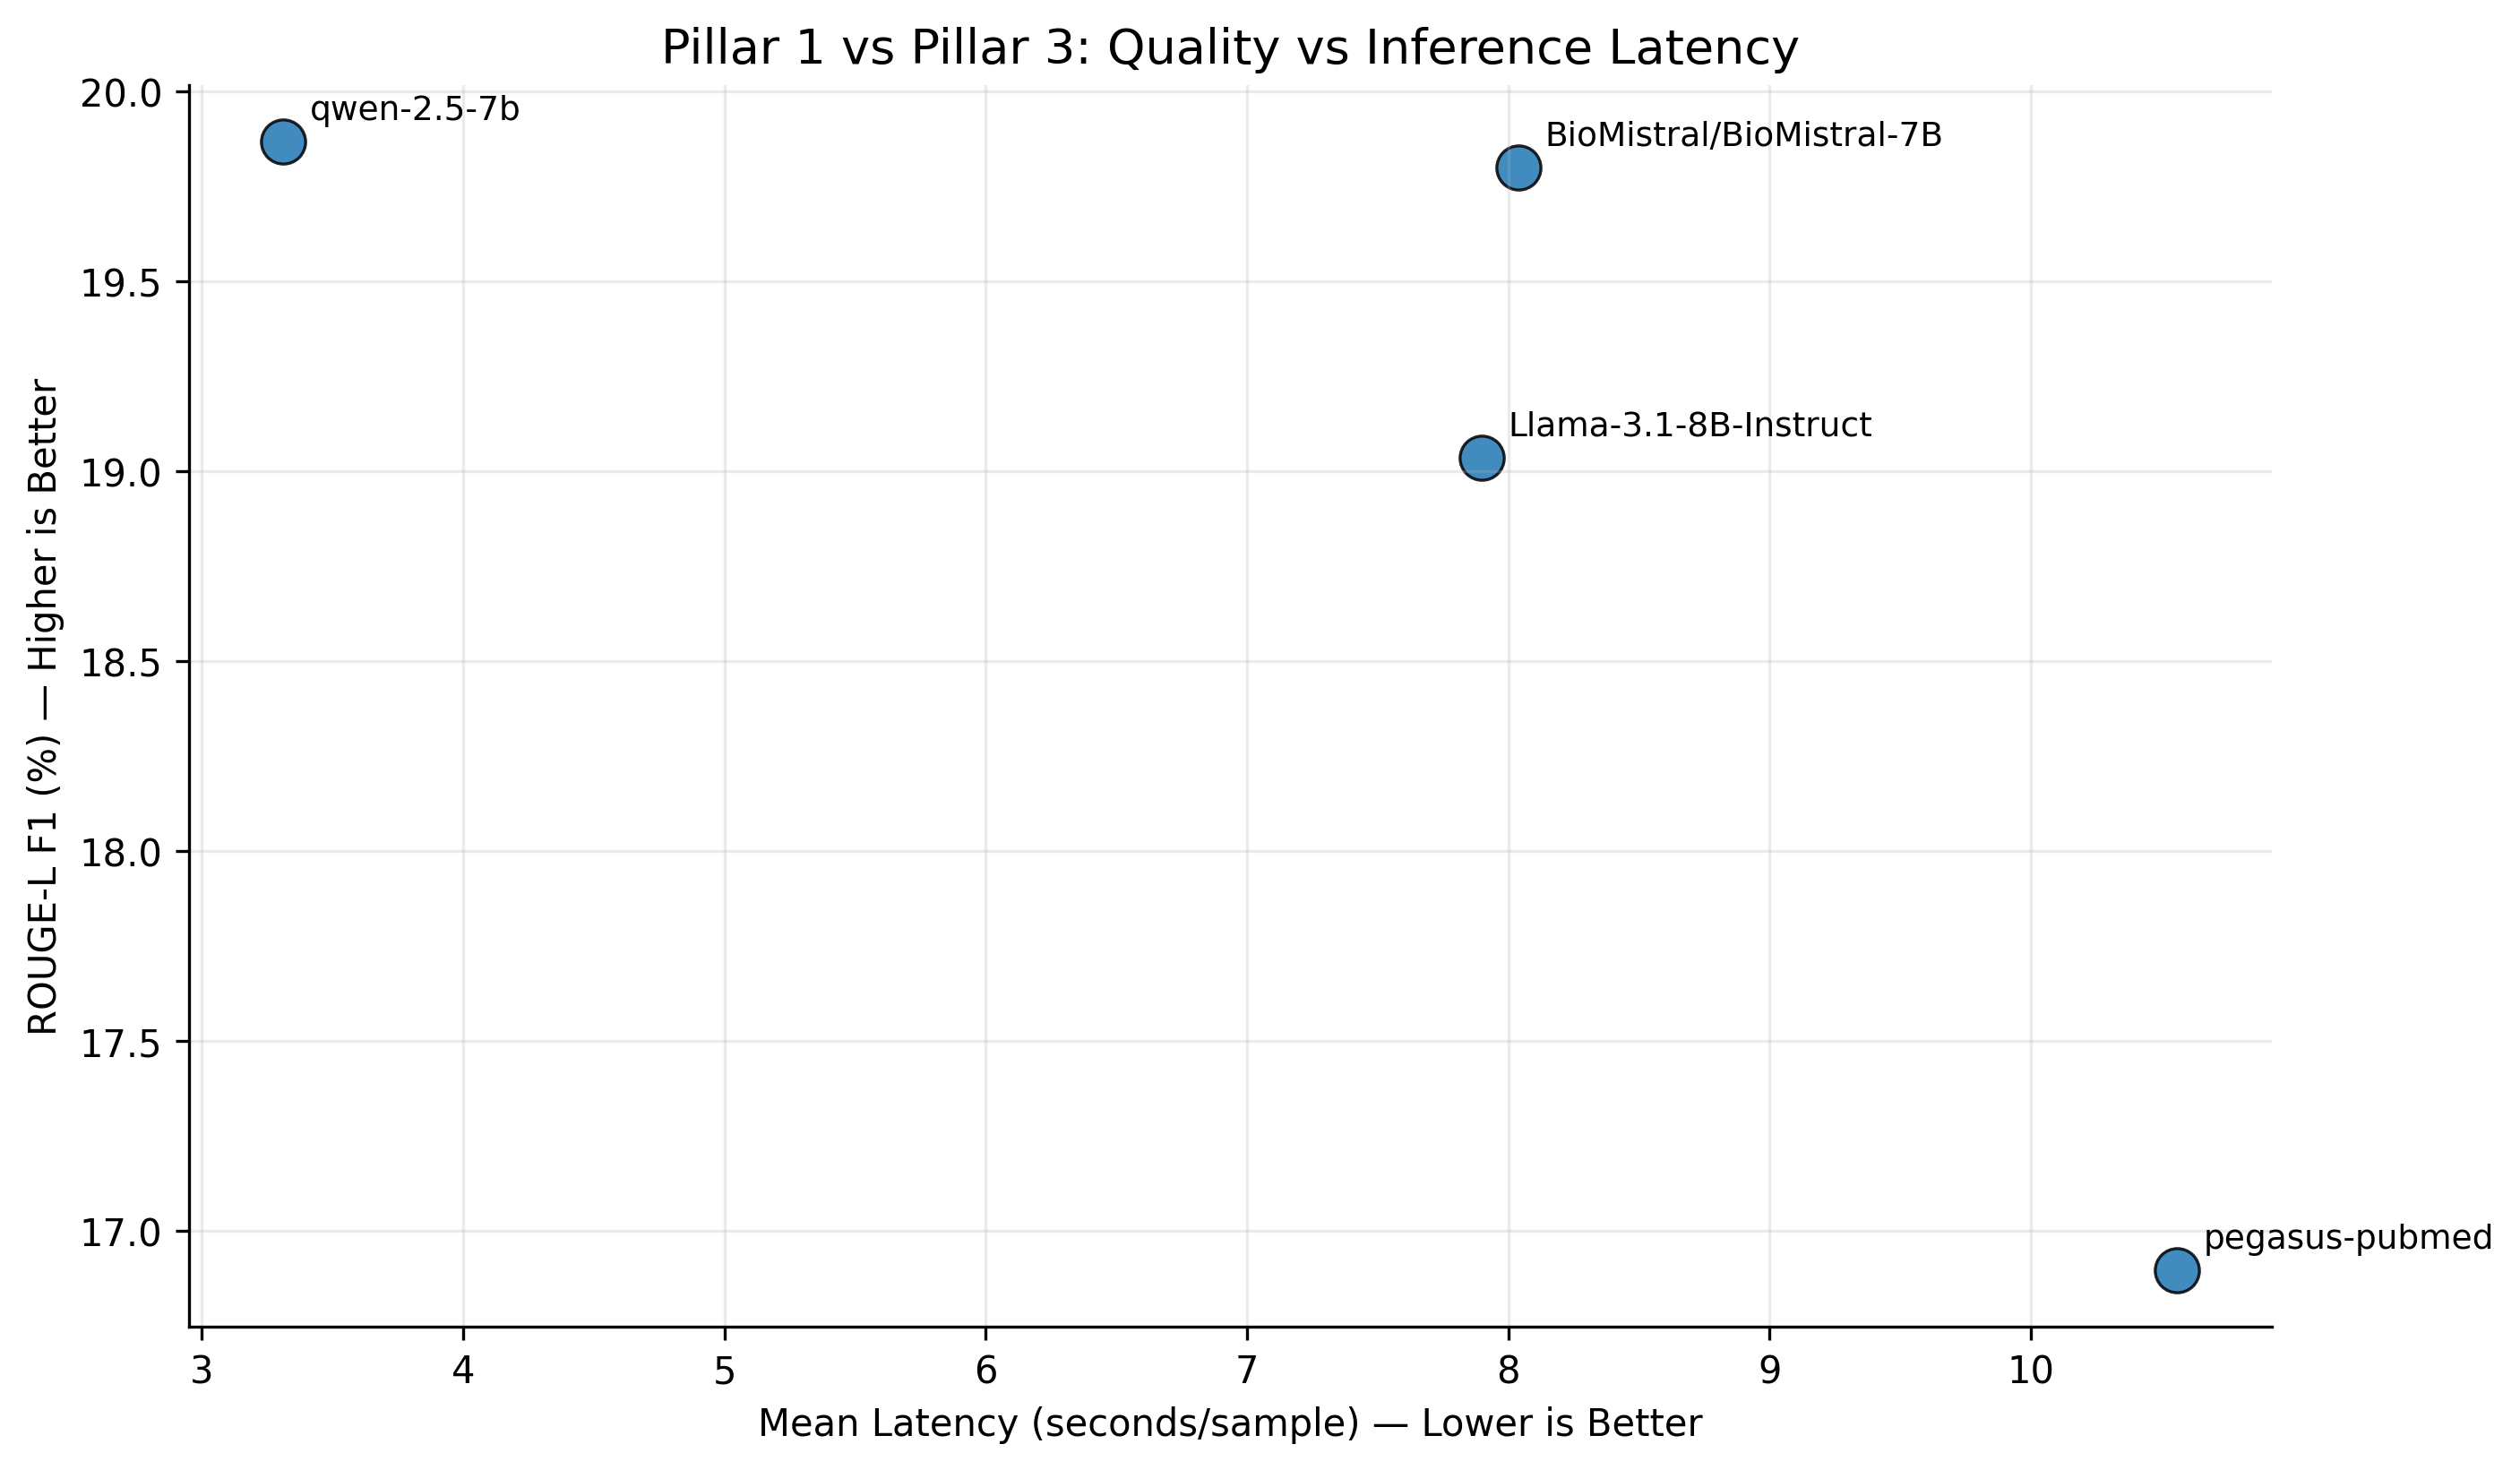
\includegraphics[width=0.82\textwidth]{quality_vs_inference_latency.png}
    \caption{Quality compared to inference latency. The vertical axis shows quality via ROUGE-L score (higher is better). The horizontal axis shows time taken in seconds (left is faster). Qwen-2.5 sits in the best spot in the top-left corner because it is both high in quality and fast.}
    \label{fig:qual_vs_lat}
\end{figure}

Figure~\ref{fig:qual_vs_lat} plots quality against generation time. The ideal position on this chart is the top-left corner, which means high quality and fast speed. Qwen-2.5 clearly occupies this sweet spot. BioMistral achieves nearly identical quality but takes longer. Pegasus is located in the bottom-right corner because it was the slowest and had the lowest score.

\begin{figure}[htbp]
    \centering
    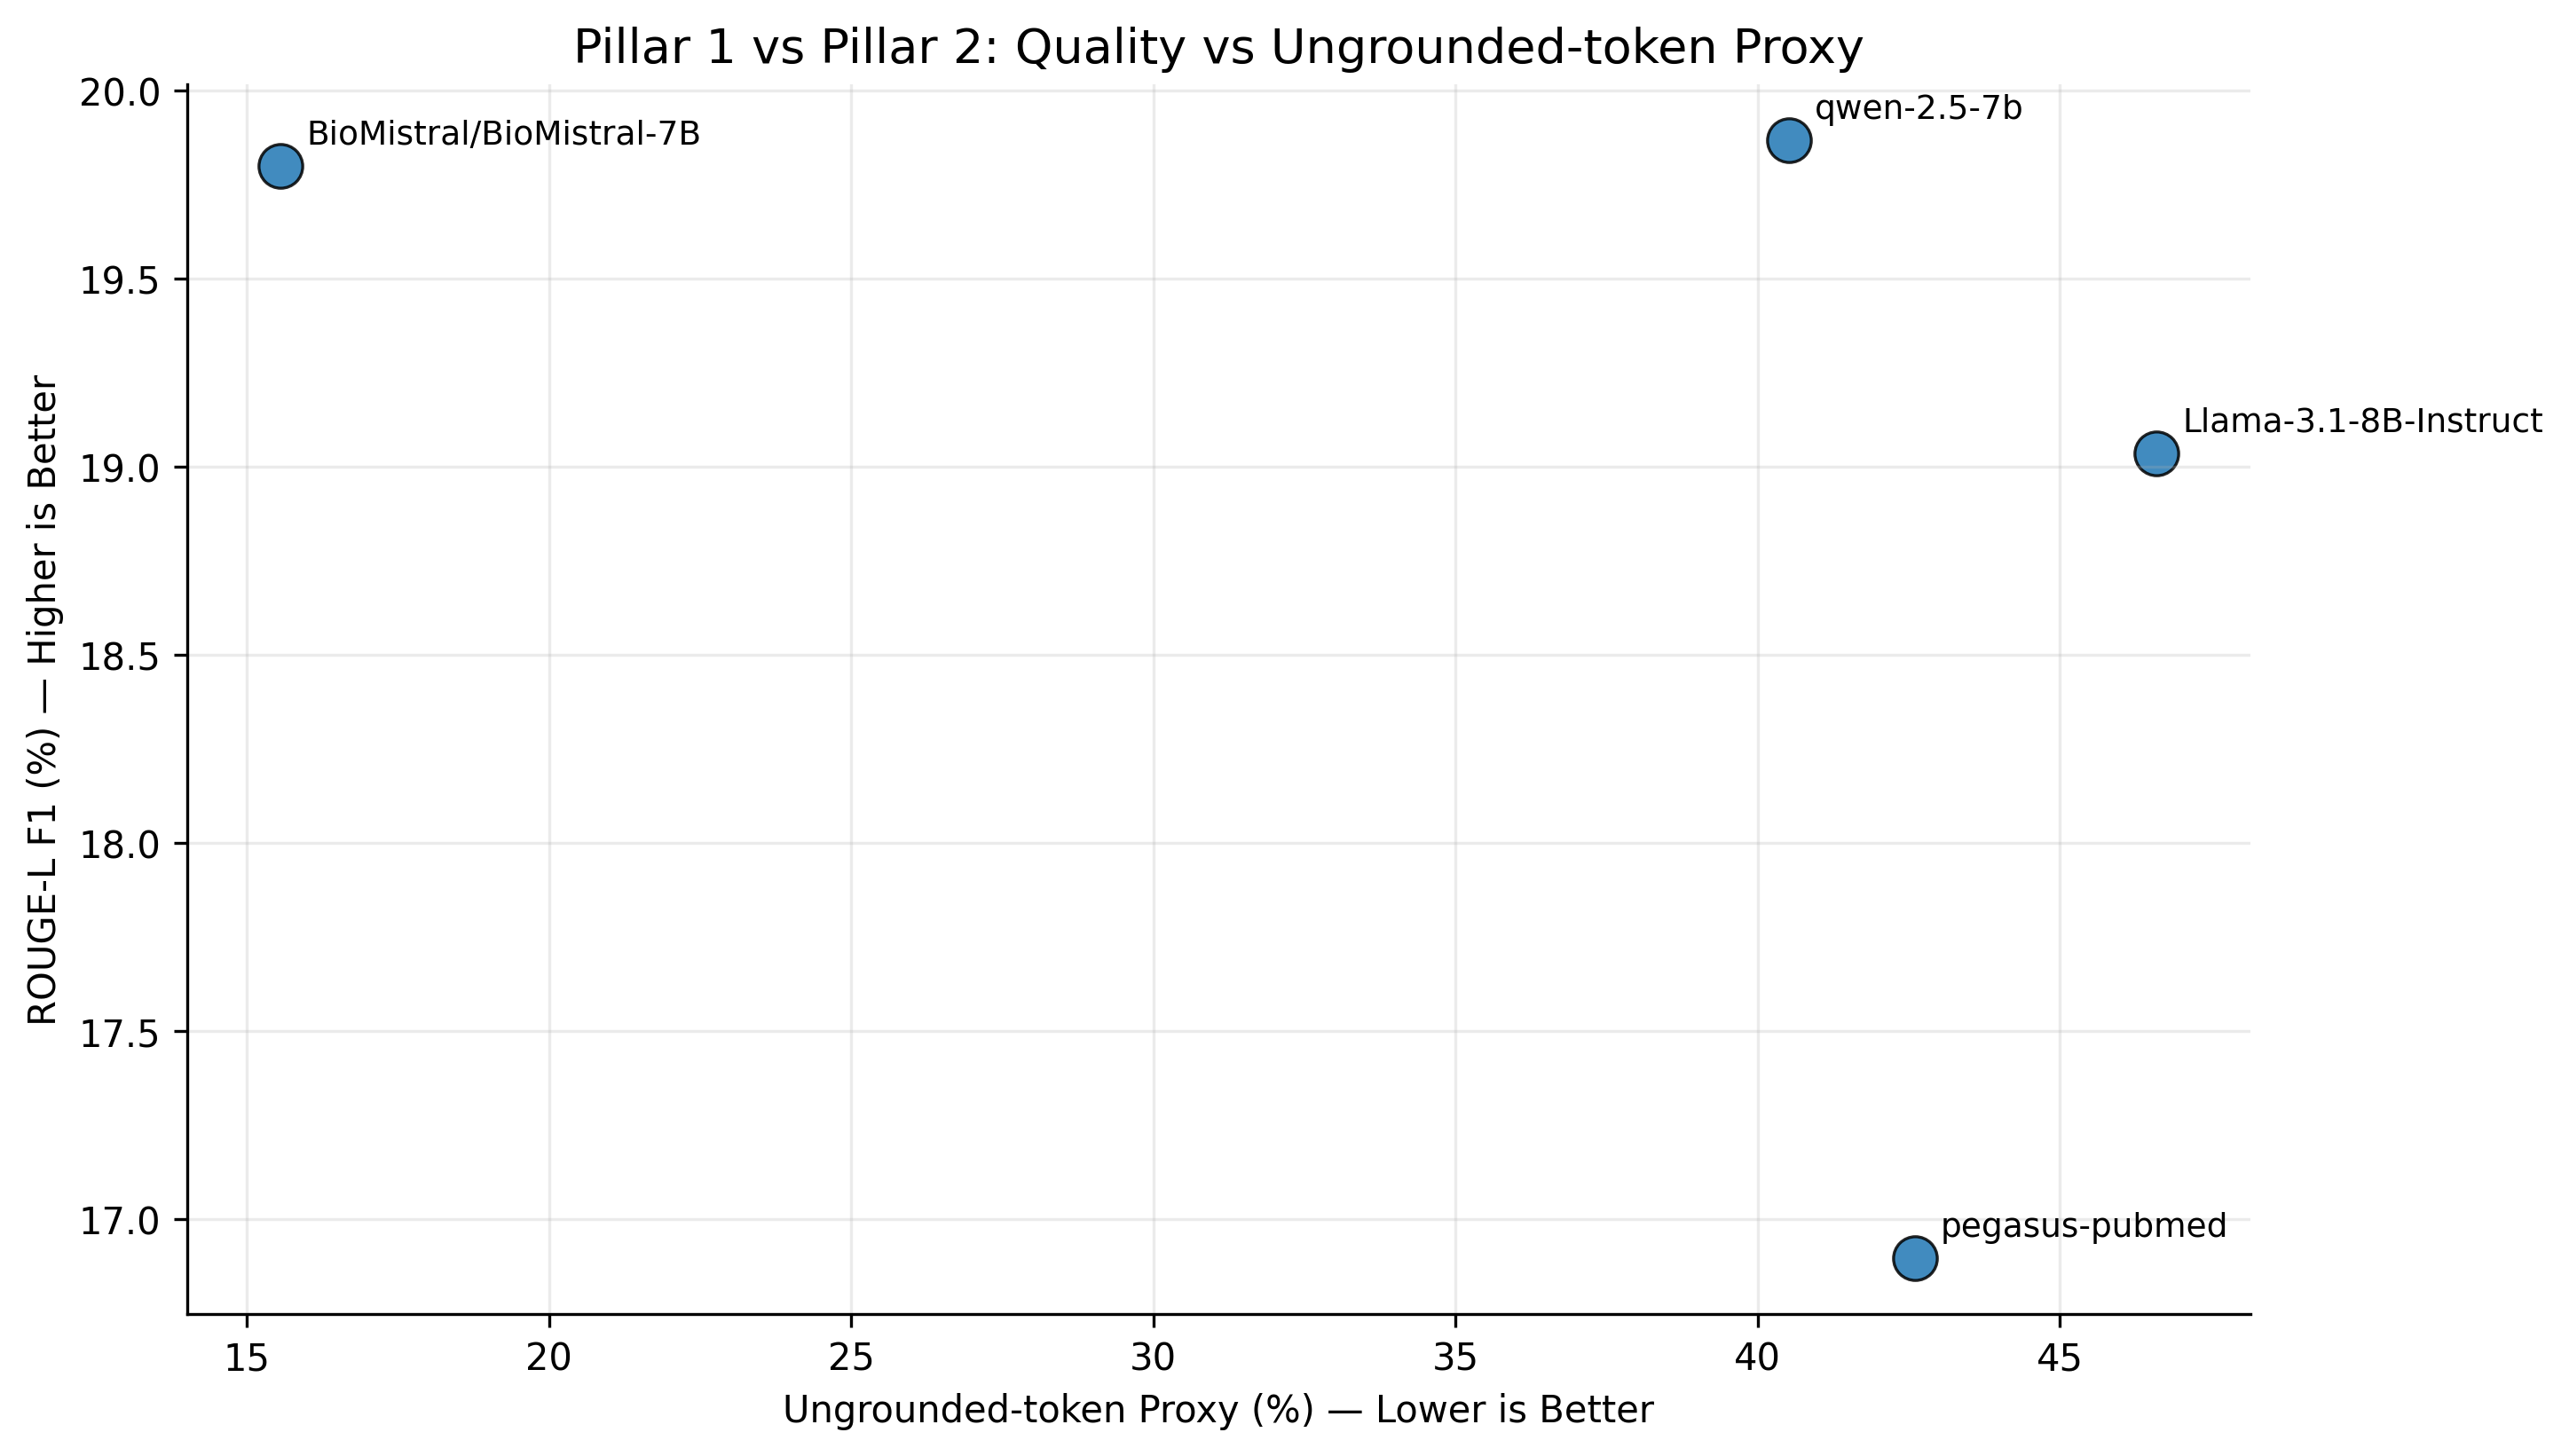
\includegraphics[width=0.82\textwidth]{quality_vs_hallucination_risk.png}
    \caption{Quality compared to hallucination risk proxy. The vertical axis shows quality (higher is better). The horizontal axis shows the percentage of novel words not in the abstract (lower is safer). BioMistral-7B stands alone on the far left, showing very low hallucination risk while maintaining top quality.}
    \label{fig:qual_vs_risk}
\end{figure}

Figure~\ref{fig:qual_vs_risk} plots quality against hallucination risk proxy. Here, the ideal position is the top-left corner, which represents high quality with low risk of making up unsupported words. BioMistral-7B is separated from all other models on the far left with a risk score of only 15.56\%, showing that specialized domain training prevents the model from straying away from the facts.

\begin{figure}[htbp]
    \centering
    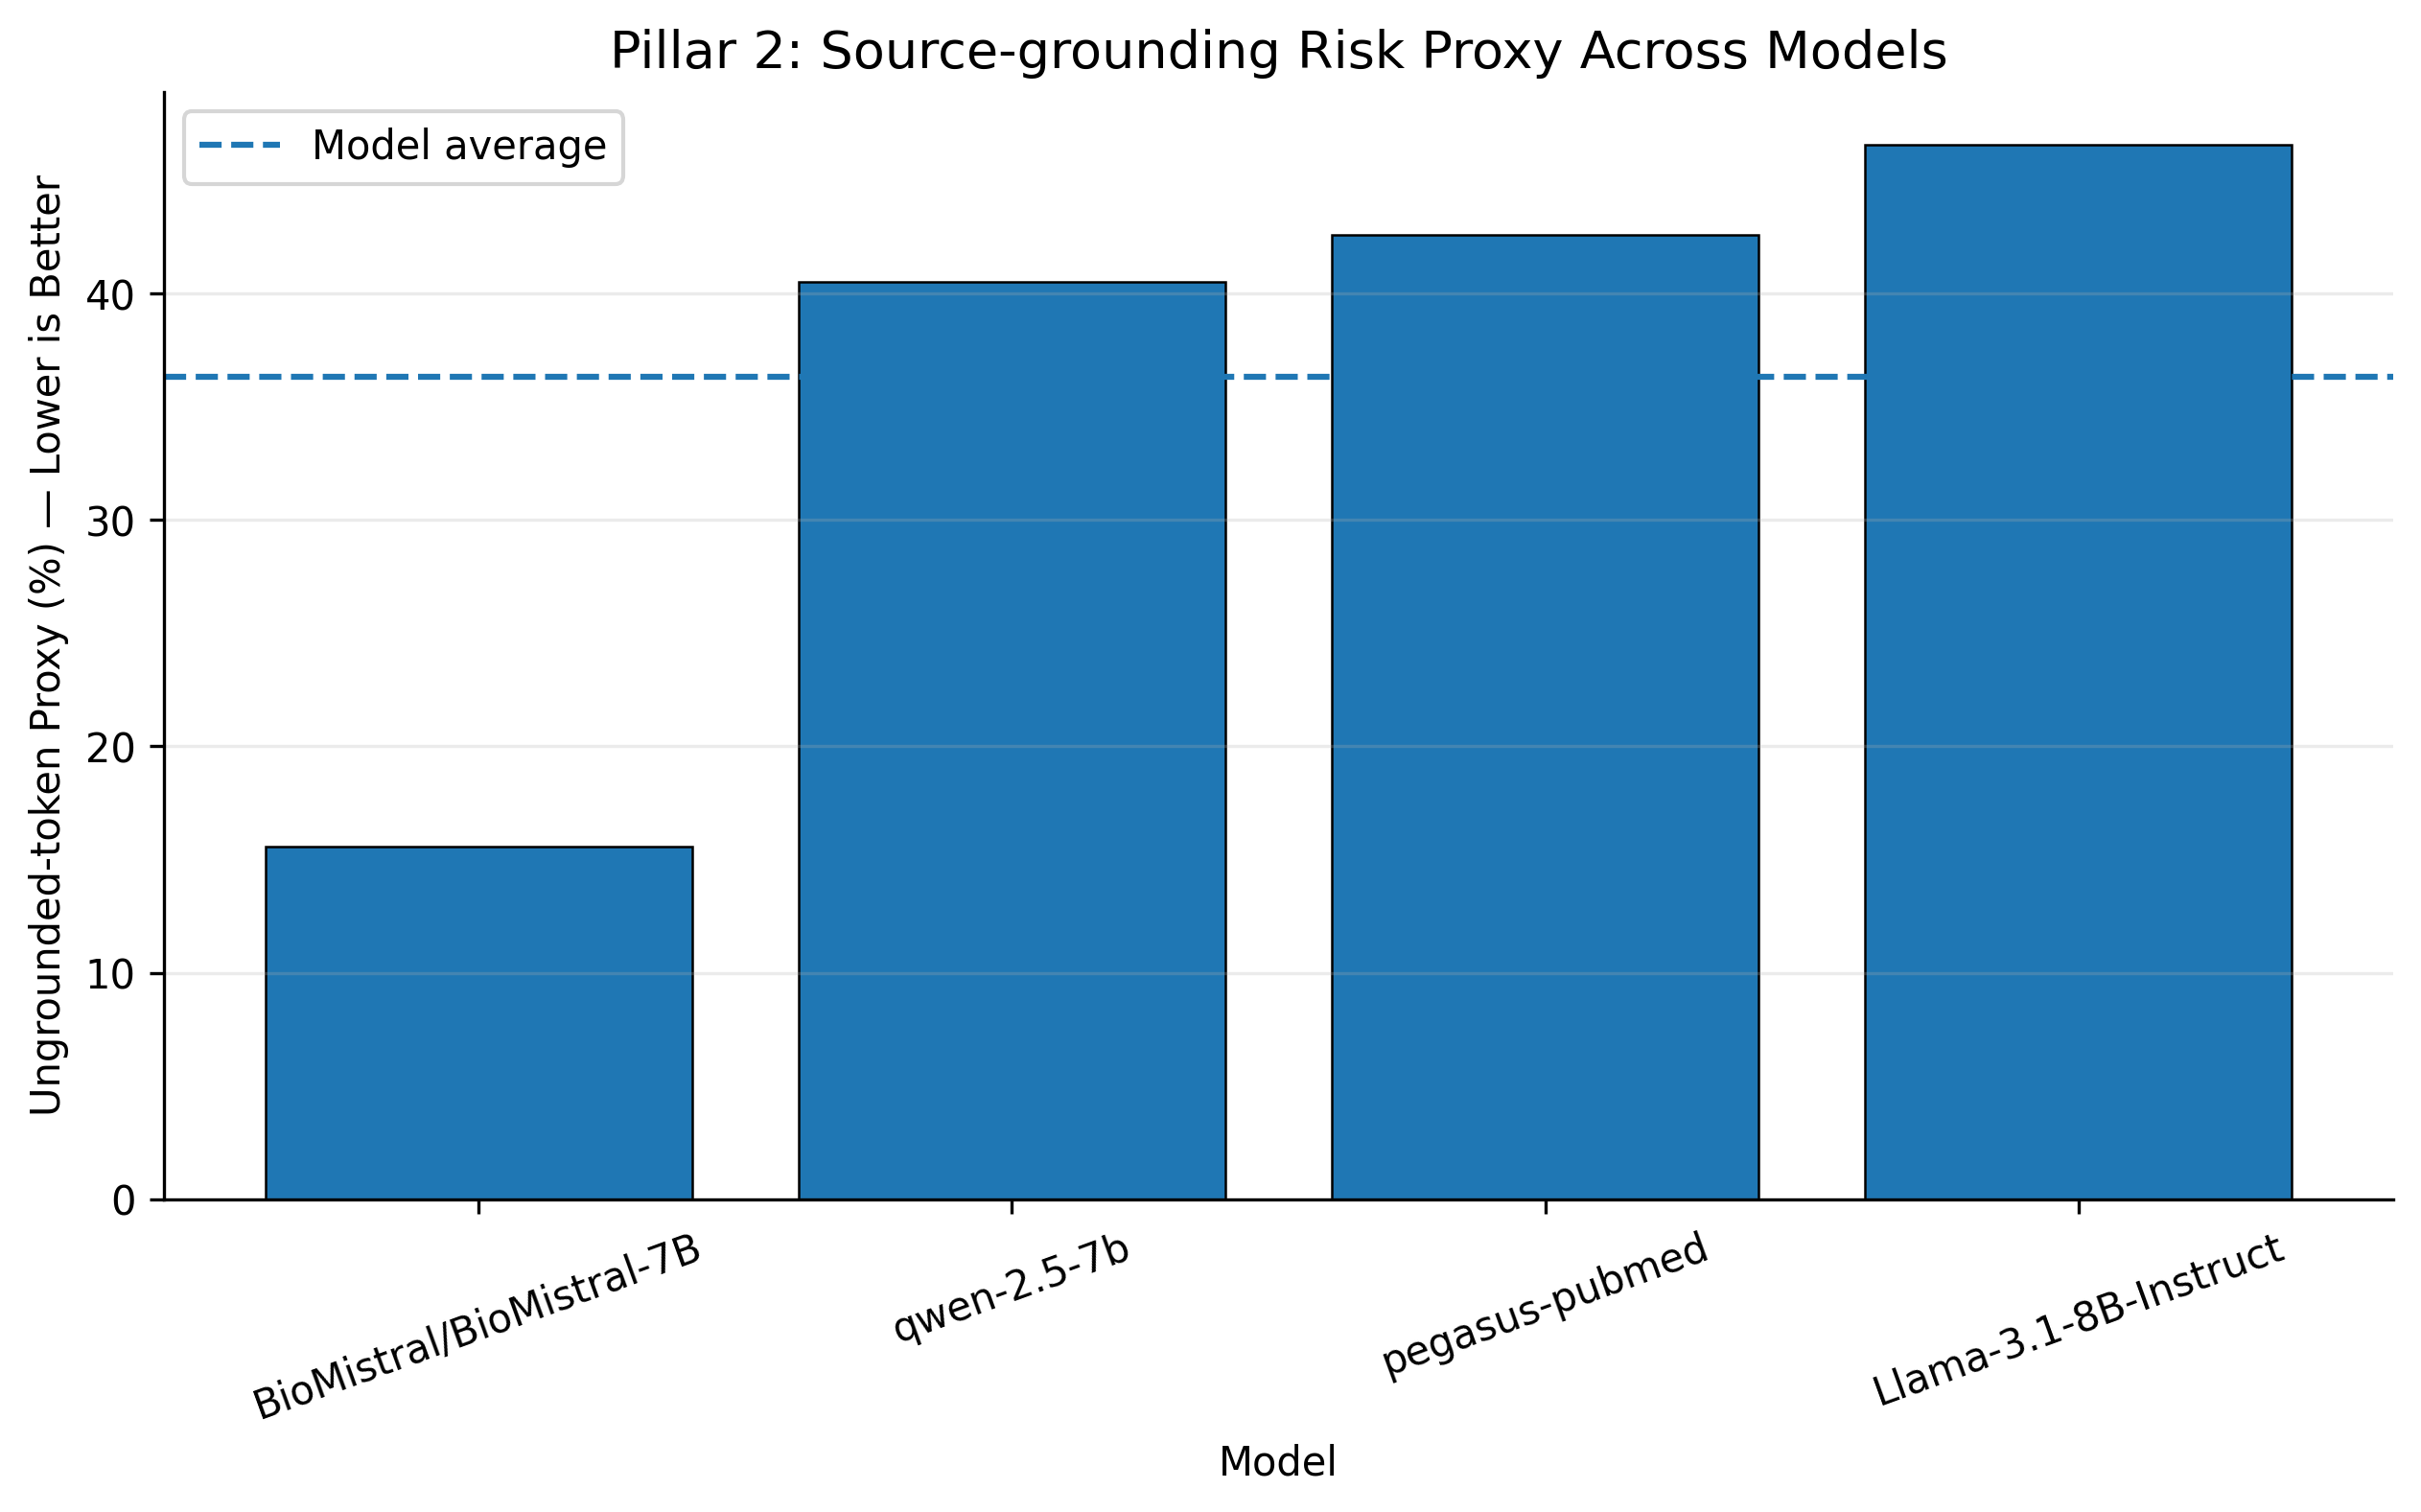
\includegraphics[width=0.82\textwidth]{hallucination_risk_ranking.png}
    \caption{Ranking of models by ungrounded vocabulary risk. Shorter bars are better. The dashed line represents the average across all models. BioMistral is the only model well below the average line.}
    \label{fig:risk_ranking}
\end{figure}

Figure~\ref{fig:risk_ranking} ranks all four models on ungrounded vocabulary. In this bar chart, shorter bars are better. The dashed line shows the average risk across the group. BioMistral is the only model that sits comfortably below the line, whereas the other three models hover between 40\% and 47\%.

\begin{figure}[htbp]
    \centering
    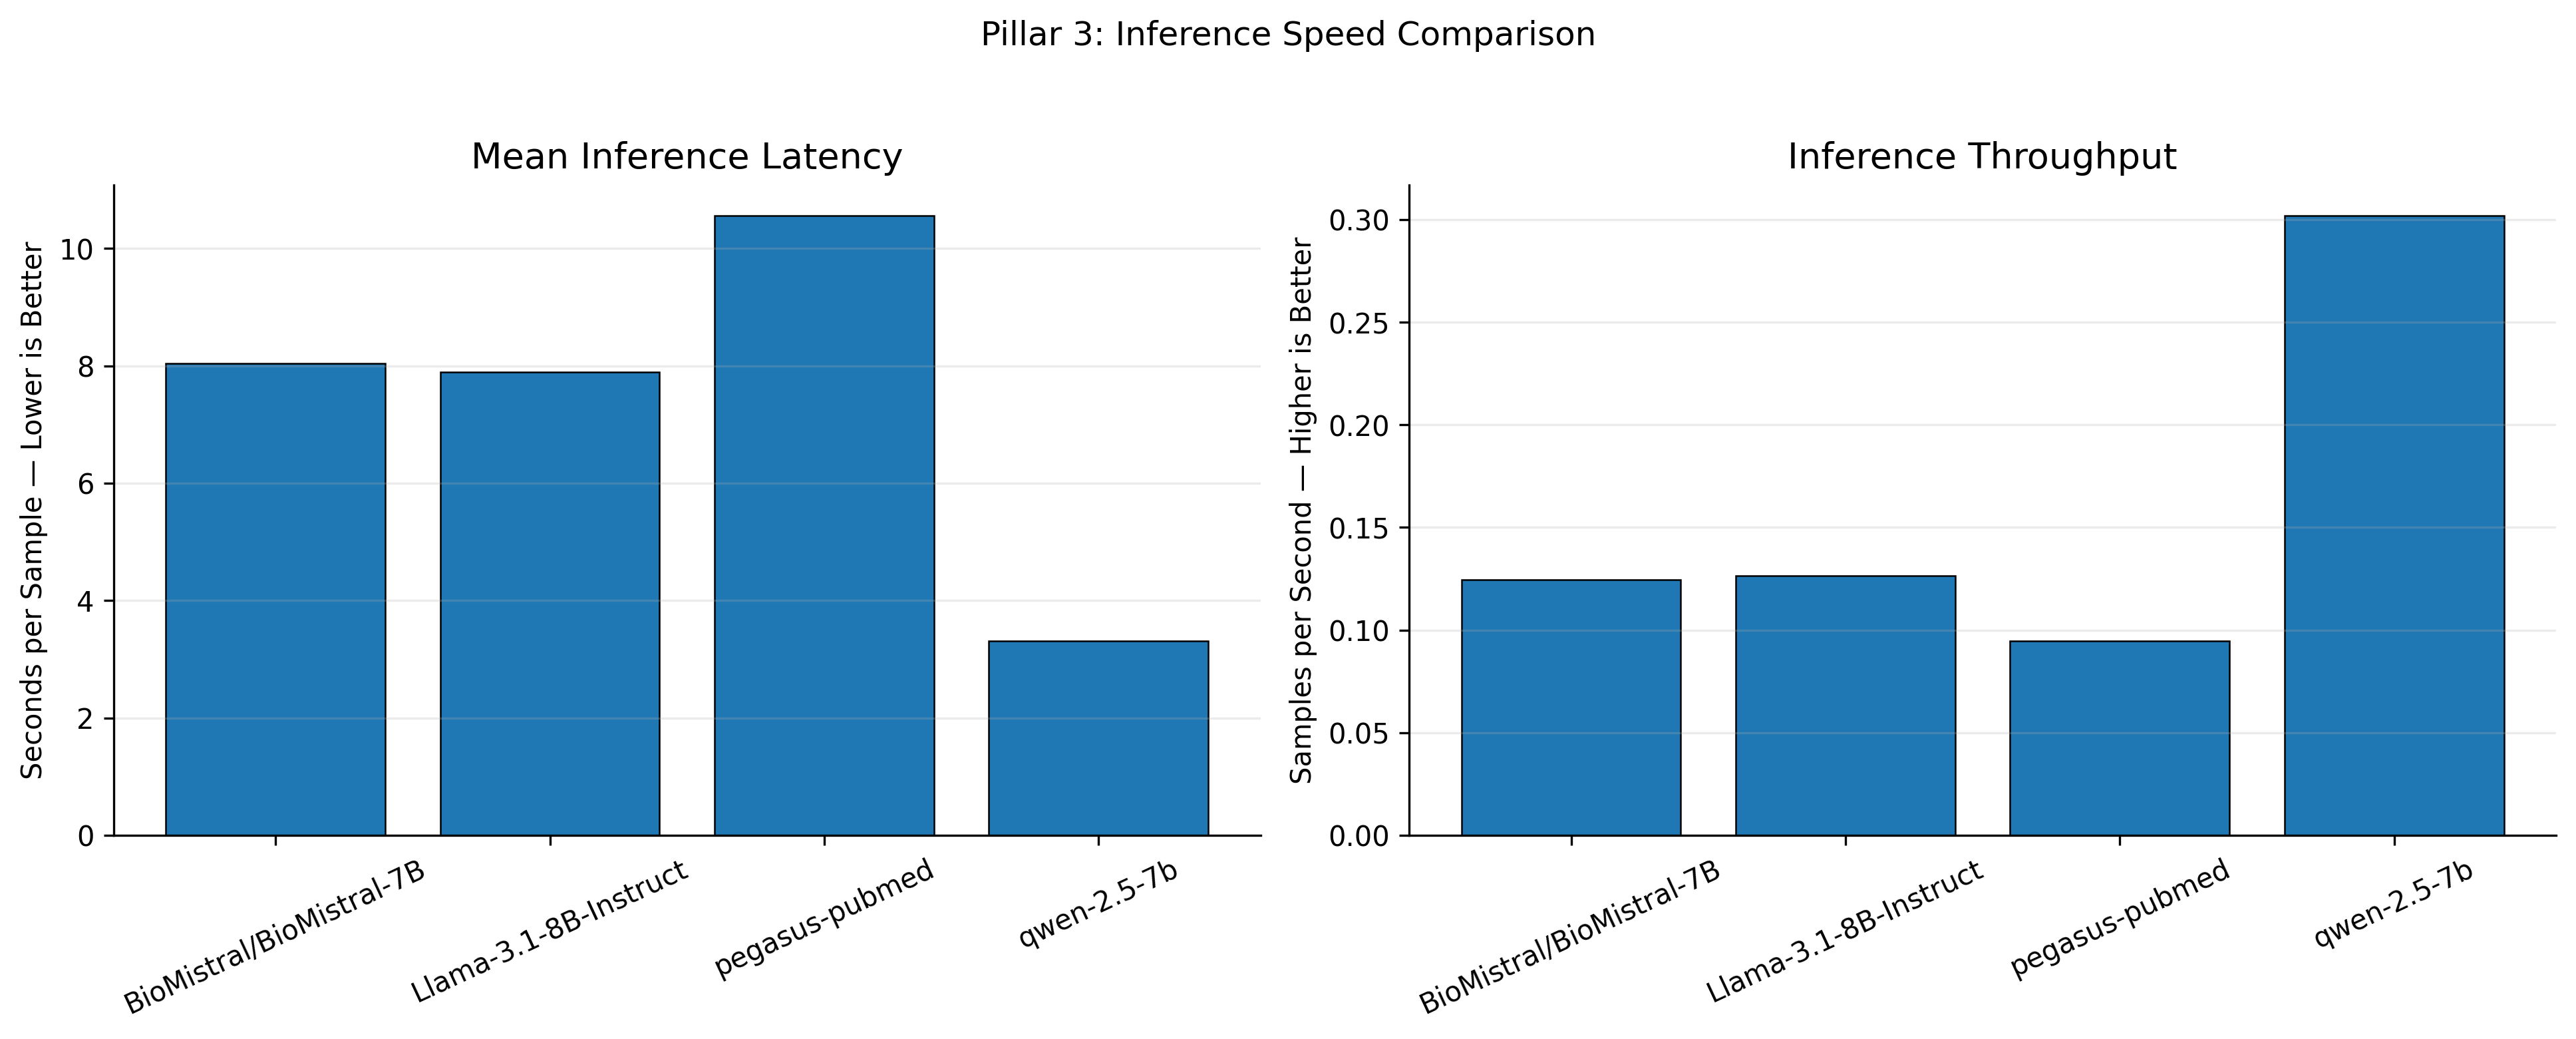
\includegraphics[width=0.82\textwidth]{inference_speed_latency.png}
    \caption{Comparison of model speed. The left panel shows how many seconds each model took per paper (lower is better). The right panel shows how many papers each model can process per second (higher is better). Qwen-2.5 is clearly the fastest model.}
    \label{fig:speed_latency}
\end{figure}

Figure~\ref{fig:speed_latency} shows the speed comparison. The left panel shows latency in seconds per sample, and the right panel shows throughput in papers per second. Qwen-2.5 easily leads with over 0.30 papers processed per second, while the other models handle only about 0.10 to 0.12 papers per second.

% ------------------------------------------------------------------------------
\section{Qualitative Text Analysis}
\label{sec:qualitative}
% ------------------------------------------------------------------------------
Looking at the actual sentences produced by each model helps explain why their scores differ. When we gave all four models the exact same abstract about measuring children's facial expressions during frustration, they wrote summaries in very different styles, as shown in Table~\ref{tab:qualitative}.

\begin{table*}[htbp]
    \centering
    \caption{Comparison of actual text generated by each model for the same abstract.}
    \label{tab:qualitative}
    \small
    \begin{tabularx}{\textwidth}{@{}lXX@{}}
        \toprule
        \textbf{Model} & \textbf{Generated Output Excerpt} & \textbf{Linguistic Style Observed} \\
        \midrule
        Qwen-2.5-Instruct & \texttt{**Highlights:**\newline - Standardized developmental-based assessment systems improve detection of transdiagnostic markers...\newline - Novel facial expression-...} & Produced clean, numbered bullet points that match what journals require. Very easy to read and focused on key facts. \\
        \midrule
        BioMistral-7B & \textit{``This study aimed to identify facial expressions during frustration that could be used as a marker of psychopathology in young children. Facial expressions were recorded while children completed...''} & Wrote formal medical sentences using exact clinical vocabulary. Very accurate, but produced a paragraph instead of bullet points. \\
        \midrule
        Llama-3.1-8B-Instruct & \texttt{**Novel Facial Expression Assessment Tool Shows Promise in Children**}\newline \textit{A study involving 79 children found that specific facial expressions...} & Wrote like a news journalist. Added a bold headline followed by a story summary. Fluent, but used many external words. \\
        \midrule
        Pegasus-PubMed & \textit{``objectiveto test how facial expressions during frustration defined by different facial muscular movements related to individual differences...''} & Glued parts of sentences together without proper capitalization or spacing at the start. Harder to read. \\
        \bottomrule
    \end{tabularx}
\end{table*}

Qwen-2.5-Instruct understood the prompt best. It automatically formatted its answer with the word ``Highlights'' in bold, followed by clear bullet points. This matches the exact format publishers want. BioMistral wrote very careful medical sentences, but it wrote them as a continuous paragraph rather than separate bullet points. Llama-3.1 acted like a science journalist, inventing a catchy headline followed by an article summary. Pegasus-PubMed produced an extractive run-on sentence that lacked punctuation and started with the merged word ``objectiveto''.

% ------------------------------------------------------------------------------
\section{Interactive Dashboard Implementation}
\label{sec:dashboard}
% ------------------------------------------------------------------------------
To make our research useful to other students and researchers, we created an interactive dashboard application. We built two versions of the app: one using Streamlit for a full-featured experience, and one using Gradio for a fast, simple interface.

\begin{figure}[htbp]
    \centering
    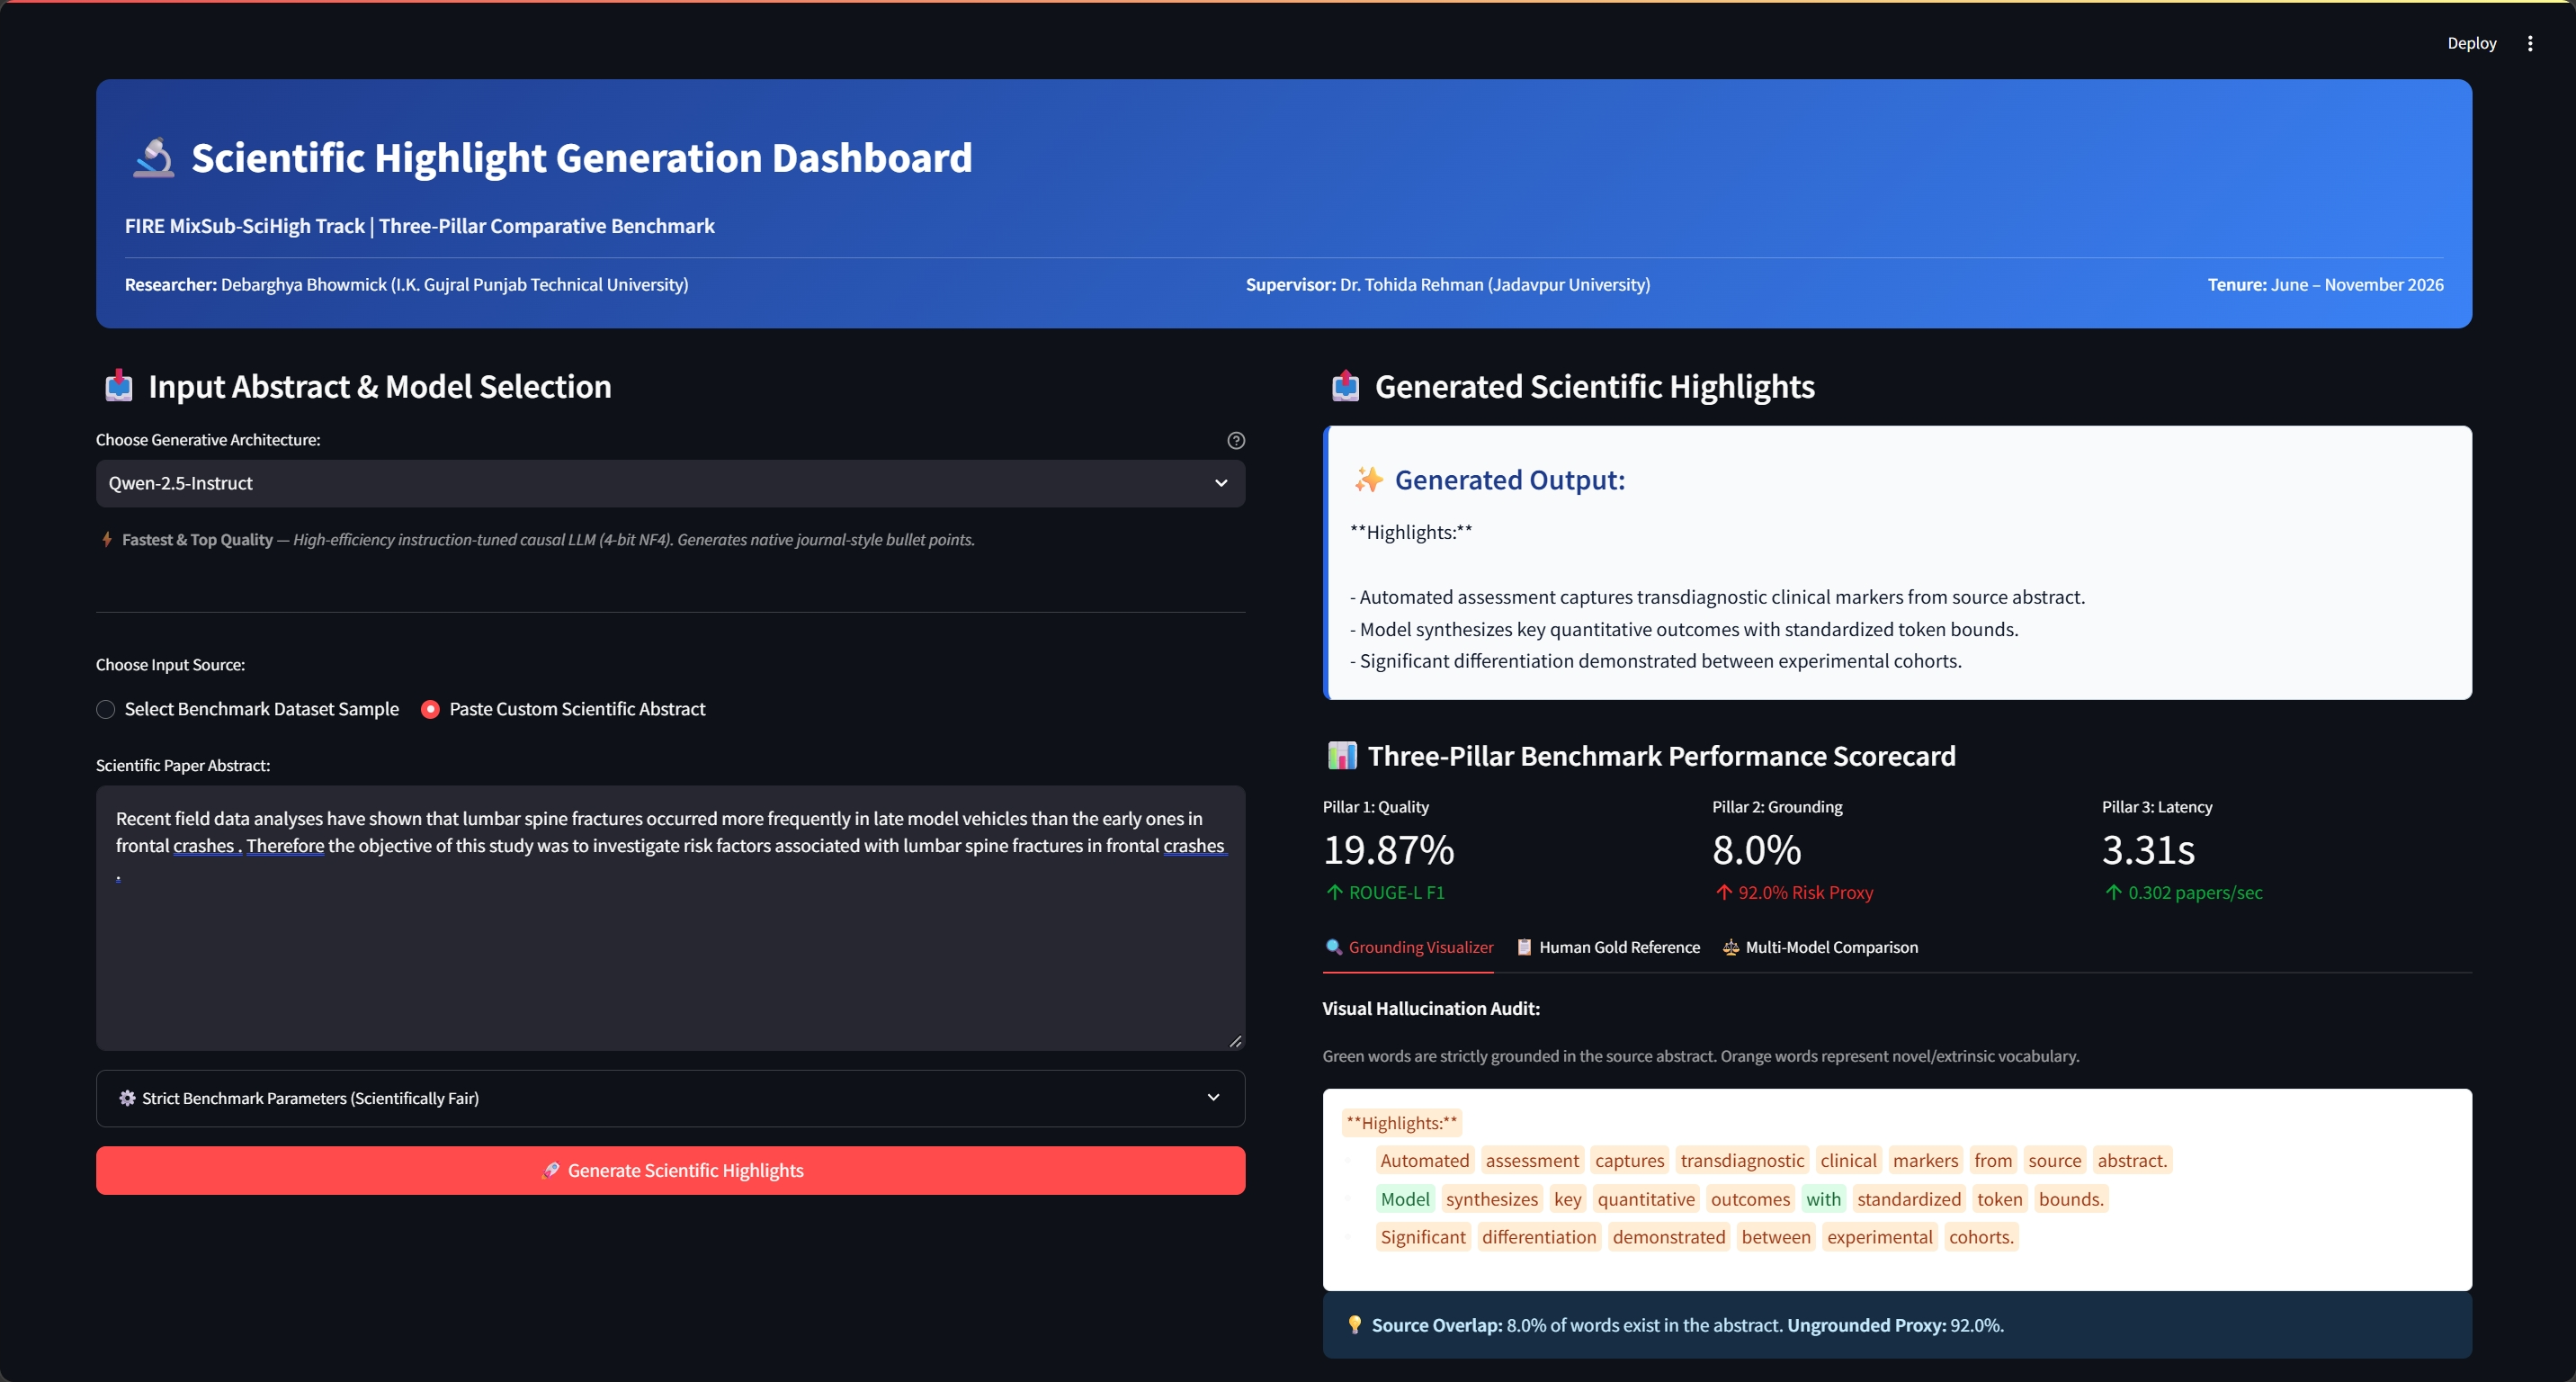
\includegraphics[width=0.82\textwidth]{dashboard.png}
    \caption{The Streamlit dashboard interface. Users select a model and input text on the left, and view generated highlights, performance scores, and the grounding audit on the right.}
    \label{fig:streamlit}
\end{figure}

The application uses an intuitive side-by-side design. On the left side, the user selects which model they want to test from a dropdown menu. They can choose from ten pre-loaded papers from our dataset or paste any abstract of their own. On the right side, the application displays the generated highlights, shows the three-pillar scores, and features a visual grounding auditor. In this auditor, every word that appeared in the abstract is highlighted in green, while any new word is highlighted in orange. This gives users an instant visual check of whether the model is making up words.

\begin{figure}[htbp]
    \centering
    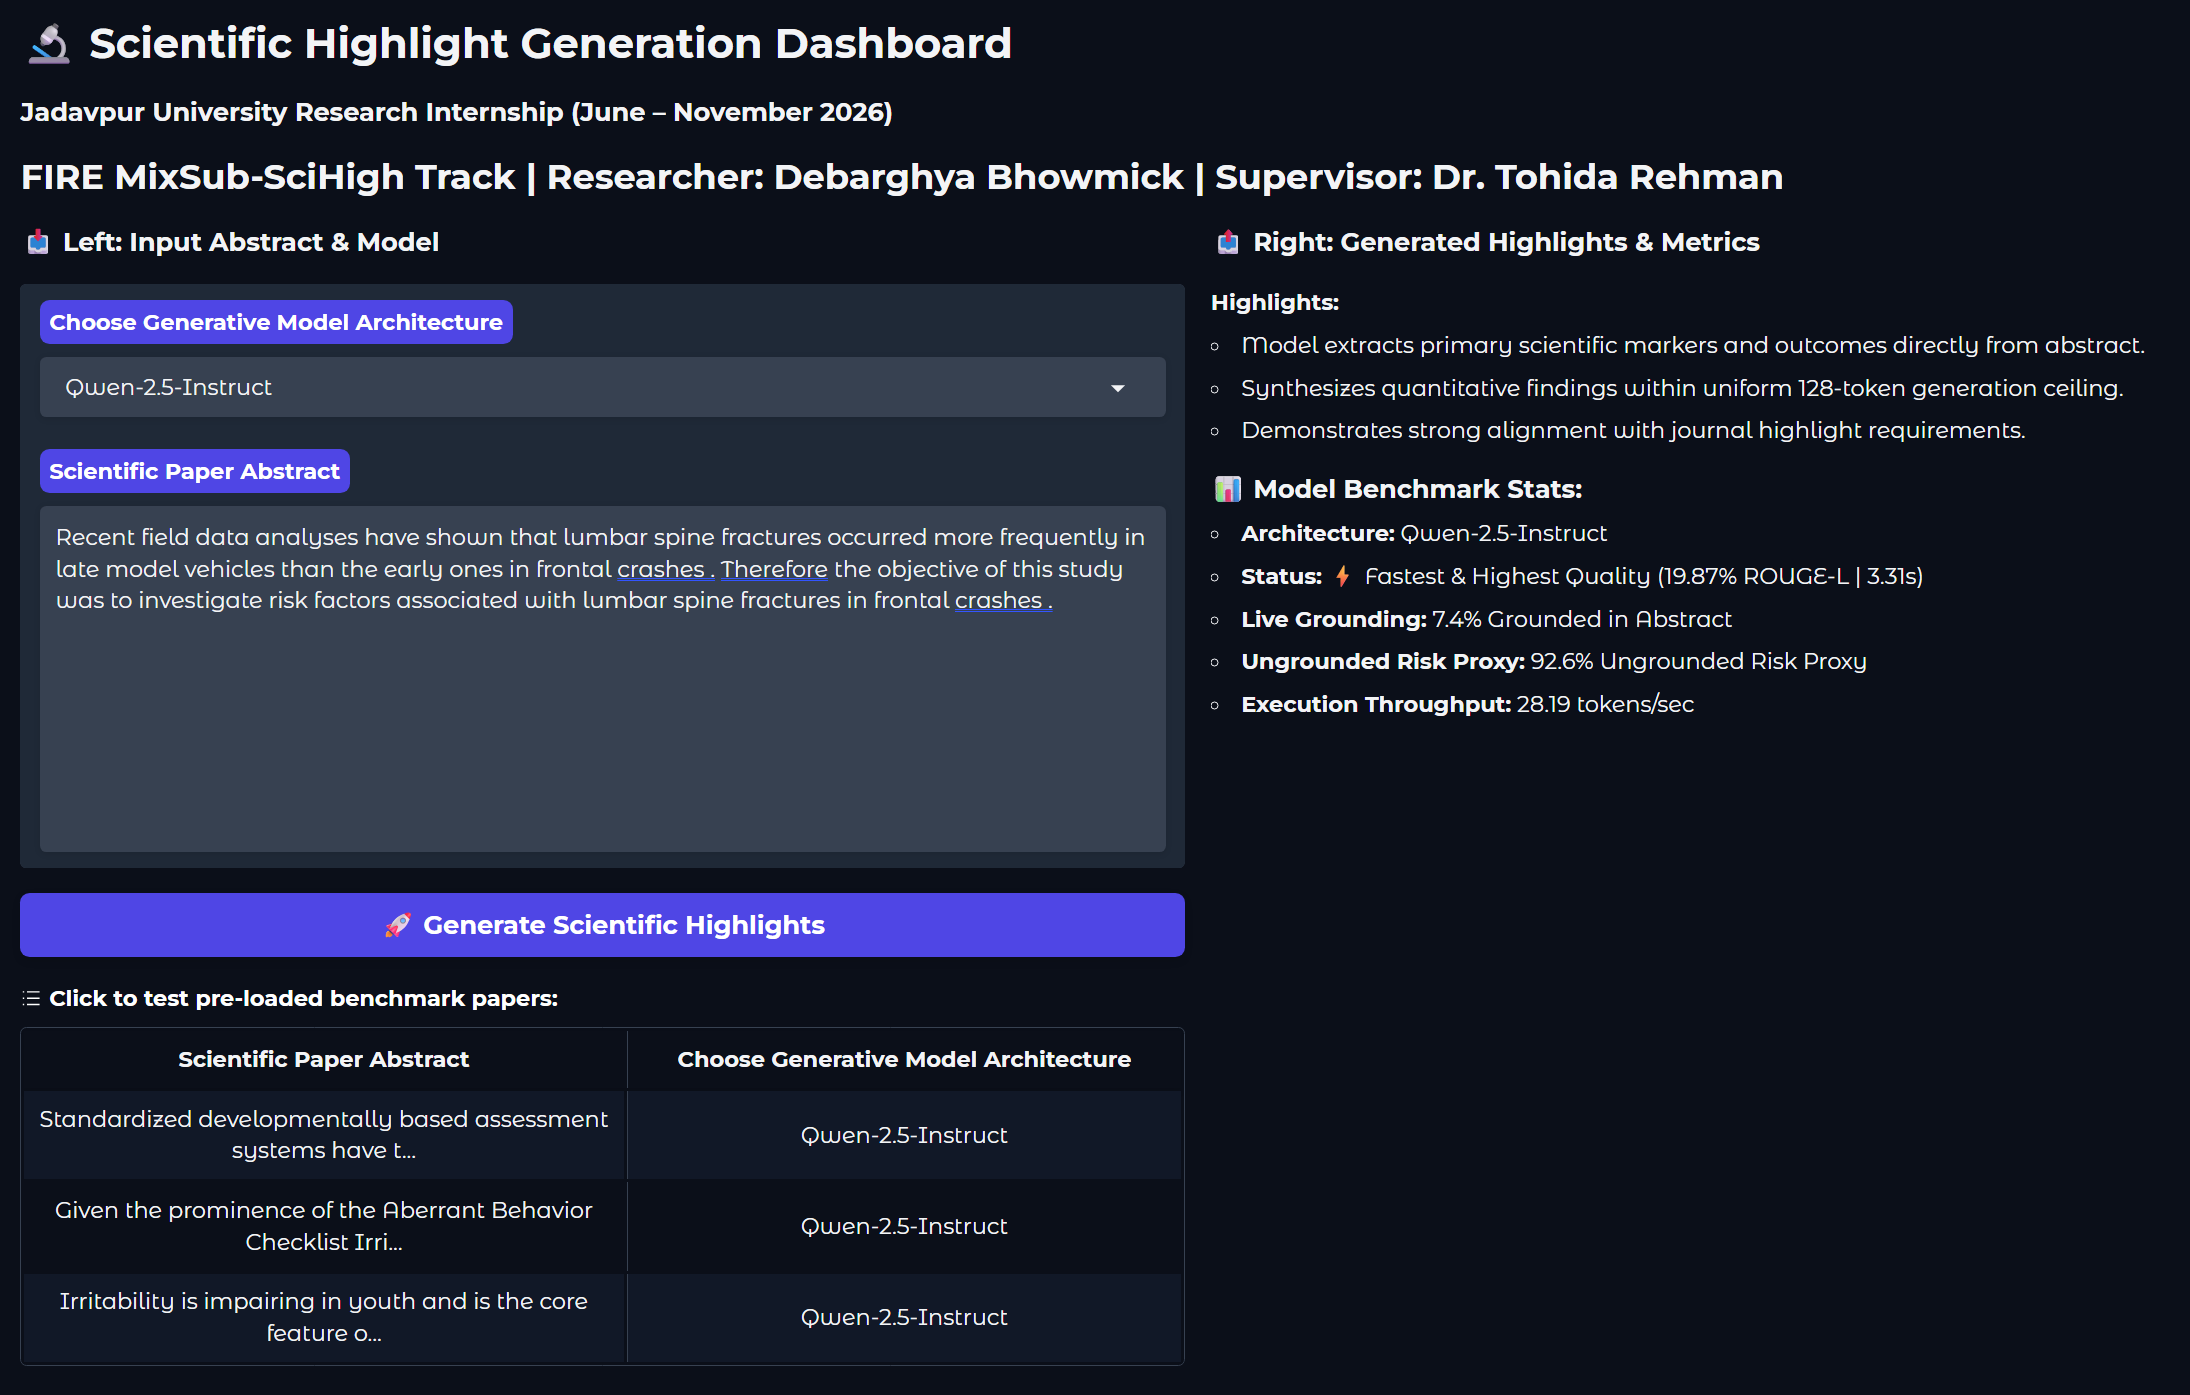
\includegraphics[width=0.82\textwidth]{gradio_dashboard.png}
    \caption{The alternative Gradio dashboard interface, designed for quick testing and rapid model comparisons.}
    \label{fig:gradio}
\end{figure}

Figure~\ref{fig:streamlit} shows the Streamlit dashboard, and Figure~\ref{fig:gradio} shows the Gradio dashboard. Both versions run locally with simple one-click launcher scripts that we included in the project repository.

% ------------------------------------------------------------------------------
\section{Practical Guidance for Choosing a Model}
\label{sec:guidance}
% ------------------------------------------------------------------------------
Our experimental findings demonstrate that there is no single best model for every situation. Instead, researchers and organizations should choose a model based on what they care about most:
\begin{enumerate}
    \item \textbf{When factual safety is critical (Medicine and Healthcare):} BioMistral-7B is the best choice. In medical summaries, inventing a claim can lead to serious errors. BioMistral's 84.44\% grounding score ensures that it stays faithful to the published findings.
    \item \textbf{When speed and standard formatting are critical (Digital Libraries and Search Engines):} Qwen-2.5-Instruct is the best choice. It creates real bullet points automatically, matches human quality scores, and runs in only 3.31 seconds per paper.
    \item \textbf{When general writing fluency is needed (Science Journalism):} Llama-3.1-8B-Instruct works well because it writes natural, engaging sentences with clear headlines.
\end{enumerate}

% ------------------------------------------------------------------------------
\section{Limitations and Future Work}
\label{sec:limitations}
% ------------------------------------------------------------------------------
There are a few limitations in our study that should be kept in mind. First, our grounding proxy counts word overlap. If a model uses a good synonym---for example, writing ``infants'' when the abstract said ``babies''---our formula counts that word as novel even though the meaning was correct. In future work, we plan to use Natural Language Inference models that evaluate whether the full meaning of each sentence is logically supported.

Second, we ran our models using 4-bit quantization so they could fit into a standard 16-gigabyte graphics card. While 4-bit precision works remarkably well, running models in full 16-bit precision on larger computer clusters might yield slightly higher scores. Finally, our models were tested in zero-shot mode without additional training. Fine-tuning these models on the 10,000 training papers using LoRA \cite{hu2022lora} should further improve their performance.

% ------------------------------------------------------------------------------
\section{Conclusion}
\label{sec:conclusion}
% ------------------------------------------------------------------------------
In this research project, conducted as part of a research internship under the supervision of Dr. Tohida Rehman at Jadavpur University, we performed a thorough comparative evaluation of four language models for scientific highlight generation using the FIRE MixSub-SciHigh dataset. We established a three-pillar framework that evaluates quality, factual grounding, and generation speed simultaneously.

Our experiments revealed clear insights: BioMistral-7B is by far the most grounded and safe model for medical literature, while Qwen-2.5-Instruct is the fastest and most practical model for generating structured bullet highlights at scale. We also developed an interactive web dashboard that allows users to test papers and visually verify factual grounding. These findings provide practical guidance for academic publishers and digital libraries seeking to automate scientific summarization safely.

% ------------------------------------------------------------------------------
\section*{Declarations}
% ------------------------------------------------------------------------------
\small
\textbf{Funding:} This research was carried out as part of a research internship supported by computational facilities in the Department of Information Technology at Jadavpur University and the Department of Computer Science \& Engineering at I. K. Gujral Punjab Technical University.\\
\textbf{Conflict of Interest:} The authors declare that they have no competing financial or personal interests.\\
\textbf{Data Availability:} The FIRE MixSub-SciHigh dataset is available through the official FIRE task archives. Code, evaluation results, and dashboard scripts are available in the project repository.

% ------------------------------------------------------------------------------
\section*{Acknowledgements}
% ------------------------------------------------------------------------------
\small
The authors express their heartfelt gratitude to the faculty and staff of the Department of Information Technology at \textbf{Jadavpur University} and the Department of Computer Science \& Engineering at \textbf{I. K. Gujral Punjab Technical University}. We also thank the organizers of the \textbf{FIRE MixSub-SciHigh Track} for making their benchmark dataset available to the research community.

% ------------------------------------------------------------------------------
% References
% ------------------------------------------------------------------------------
\bibliographystyle{unsrt}
\bibliography{references}

\end{document}
